\documentclass[11pt,a4paper]{article}

\usepackage[utf8]{inputenc}
\usepackage[T1]{fontenc}
\usepackage{amsmath,amssymb,amsthm}
\usepackage{booktabs}
\usepackage{graphicx}
\usepackage{hyperref}
\usepackage[margin=1in]{geometry}

\newtheorem{theorem}{Theorem}
\newtheorem{corollary}[theorem]{Corollary}
\newtheorem{conjecture}[theorem]{Conjecture}
\newtheorem{definition}[theorem]{Definition}

\title{\textbf{Carry-Optimal Goldbach Partitions, Lemoine Verification to $10^{12}$, and Information-Theoretic Structure of Minimal Prime Witnesses}}
\author{Joseph Jonathan Fernandes\\
\texttt{https://github.com/JosephJonathanFernandes/goldbach-simd}}
\date{2026}

\begin{document}
\maketitle

\begin{abstract}
We introduce the \emph{Goldbach Binary Carry Excess} $\Delta_c^*(n) = \min_{p+q=n} \operatorname{carries}(p, q) - v_2(n)$, measuring the minimum number of binary carries beyond the unavoidable $2$-adic lower bound $v_2(n)$ required to express an even integer $n \ge 6$ as a sum of two odd primes. We prove an exact bit-level characterization: $\Delta_c^*(n) = 0$ if and only if $p = 1 \mathbin{|} s$ and $q = 1 \mathbin{|} ((n - 2) \oplus s)$ for some proper binary submask $s \subset n - 2$. As immediate corollaries, we establish infinite exception families at binary weight $w = \operatorname{popcount}(n - 2) \in \{1, 2\}$ linked directly to Fermat primes. Using exact submask enumeration across all $5 \times 10^8$ even integers up to $10^9$, we observe a sharp phase transition in $w$: carry-optimality rises to $99.5972\%$ at $10^9$, with a single exception at $w = 12$ ($n = 743{,}309{,}774 = \texttt{0x2C4E01CE}$ out of $50.78$ million integers) and zero exceptions across all $378.76$ million integers with $w \ge 13$. Alongside this result, we present a cache-blocked AVX2 segmented bucket sieve engine achieving $4.33 \times 10^9$ even numbers/sec, which we apply to verify Lemoine's conjecture ($n = p + 2q$) deterministically to $10^{12}$, Twin-Prime Goldbach to $10^{10}$, and the information-theoretic structure of minimal Goldbach witnesses across $5 \times 10^9$ even integers.
\end{abstract}

\section{Introduction}
The binary Goldbach conjecture—verified up to $4 \times 10^{18}$ by Oliveira e Silva, Herzog, and Pardi~\cite{oliveira2014}—asserts that every even integer $n \ge 4$ is the sum of two primes. In this paper we study Goldbach partitions through two complementary computer-science lenses: (i) the \emph{binary hardware carry complexity} of adding two primes $p + q = n$, and (ii) the \emph{information-theoretic structure} of the minimal prime witness stream $\{p_{\min}(2k)\}$.

\section{Carry-Optimal Goldbach Partitions}

\begin{definition}[Binary Carry Count and Carry Excess]
For positive integers $p, q$, let $\operatorname{pop}(x)$ denote the binary Hamming weight (number of $1$-bits) of $x$ and $v_2(n)$ the $2$-adic valuation (number of trailing zeros in binary). By Kummer's theorem~\cite{kummer1852} in base $2$, the total number of carries generated during the binary addition $p + q$ is
\begin{equation}
\operatorname{carries}(p, q) = \operatorname{pop}(p) + \operatorname{pop}(q) - \operatorname{pop}(p + q).
\end{equation}
For an even integer $n \ge 6$, we define the \emph{global Goldbach carry excess} as
\begin{equation}
\Delta_c^*(n) = \min_{\substack{p + q = n \\ p, q \text{ odd prime}}} \operatorname{carries}(p, q) - v_2(n).
\end{equation}
We call $n$ \emph{carry-optimal} if $\Delta_c^*(n) = 0$.
\end{definition}

\begin{theorem}[Exact Submask Characterization]
\label{thm:submask}
Let $n \ge 6$ be even with $k = v_2(n) \ge 1$, and let $M = n - 2$. For any odd integers $p, q \ge 1$ with $p + q = n$:
\begin{enumerate}
    \item $\operatorname{carries}(p, q) \ge k$, and
    \item $\operatorname{carries}(p, q) = k$ if and only if there exists a binary submask $s \subseteq M$ (i.e., $s \mathbin{\&} M = s$) such that
    \begin{equation}
    p = 1 \mathbin{|} s \qquad\text{and}\qquad q = 1 \mathbin{|} (M \oplus s).
    \end{equation}
\end{enumerate}
\end{theorem}

\begin{proof}
Write $n = H + 2^k$ where all $1$-bits of $H$ lie strictly above bit position $k$. Since $p$ and $q$ are odd, $p_0 = q_0 = 1$, producing carry $c_1 = 1$. For each bit position $1 \le j \le k - 1$, $n_j = 0$ and incoming carry $c_j = 1$ force $p_j + q_j = 1$, which propagates $c_{j+1} = 1$. Thus bits $0, \dots, k-1$ always generate at least $k$ carries, proving (1).

Equality $\operatorname{carries}(p, q) = k$ holds if and only if no further carries occur ($c_j = 0$ for all $j \ge k + 1$). At bit $k$, $n_k = 1$ and $c_k = 1$ force $p_k = q_k = 0$ to absorb the incoming carry with $c_{k+1} = 0$. For every bit $j > k$ with $c_j = 0$, avoiding $c_{j+1} = 1$ requires $p_j = q_j = 0$ whenever $n_j = 0$, and $p_j \oplus q_j = 1$ whenever $n_j = 1$. Combining bit ranges $\{1, \dots, k-1\}$ (mask $2^k - 2$) and $\{j > k : n_j = 1\}$ (mask $H$) yields the disjoint union $M = H \mathbin{|} (2^k - 2) = n - 2$, so $p - 1$ and $q - 1$ partition the $1$-bits of $M$ disjointly. Conversely, any submask $s \subseteq M$ gives $p + q = 2 + s + (M - s) = n$ and $\operatorname{pop}(p) + \operatorname{pop}(q) = 2 + \operatorname{pop}(M) = 2 + (\operatorname{pop}(n) - 1) + (k - 1) = \operatorname{pop}(n) + k$, hence $\operatorname{carries}(p, q) = k$.
\end{proof}

\begin{corollary}[Infinite Exception Families and Fermat Primes]
Let $w = \operatorname{pop}(n - 2)$. There are exactly $2^{w-1} - 1$ unordered odd pairs $\{p, q\}$ with $p, q > 1$ achieving $\operatorname{carries}(p, q) = v_2(n)$. In particular:
\begin{enumerate}
    \item If $w = 1$ (i.e., $n = 2^a + 2$ for $a \ge 2$), there are zero valid pairs, so $\Delta_c^*(2^a + 2) \ge 1$ unconditionally.
    \item If $w = 2$ and $n = 2^a + 2^b + 2$ ($a > b \ge 2$), the unique valid pair is $(2^b + 1, 2^a + 1)$; hence $\Delta_c^*(n) = 0$ if and only if both $2^a + 1$ and $2^b + 1$ are Fermat primes.
\end{enumerate}
\end{corollary}

\begin{theorem}[Unconditional Infinite Exceptions for Every Weight $w \ge 1$ and $\Omega(\ln \ln N)$ Lower Bound]
\label{thm:allw}
For every integer $w \ge 1$, there exist infinitely many even integers $n$ with $\operatorname{pop}(n - 2) = w$ and $\Delta_c^*(n) \ge 1$ (in fact, having \emph{both} $p = 1 \mathbin{|} s$ and $q = 1 \mathbin{|} ((n-2) \oplus s)$ strictly composite for every proper non-empty submask $s \subset n - 2$). Explicitly, let
\begin{equation}
L_w = \operatorname{lcm}\bigl\{\operatorname{ord}_\ell(2) : \ell \text{ prime},\; 3 \le \ell \le 2w - 1\bigr\}
\end{equation}
(with $L_1 = 1$). Then for any strictly increasing integers $k_1 < k_2 < \dots < k_w$ satisfying $2^{k_1 L_w + 1} > 2w - 1$, the integer $n = 2 + \sum_{i=1}^w 2^{k_i L_w + 1}$ satisfies $\operatorname{pop}(n - 2) = w$ and $\Delta_c^*(n) \ge 1$. Moreover, defining $W_{\max}(N) = \max\{\operatorname{pop}(n - 2) : 6 \le n \le N \text{ even},\; \Delta_c^*(n) > 0\}$, we have unconditionally for all sufficiently large $N$:
\begin{equation}
W_{\max}(N) \ge \Bigl(\frac{1}{2} - o(1)\Bigr) \ln \ln N.
\end{equation}
\end{theorem}

\begin{proof}
For $w = 1$ the claim follows from Corollary~2. Let $w \ge 2$ and let $s \subset M = n - 2$ be any non-empty proper submask of Hamming weight $r = \operatorname{pop}(s) \in \{1, \dots, w - 1\}$. Then $2r + 1$ is an odd integer satisfying $3 \le 2r + 1 \le 2w - 1$, so it possesses at least one odd prime factor $\ell \le 2w - 1$. Because $\operatorname{ord}_\ell(2) \mid L_w$, every bit of $M$ satisfies $2^{k_i L_w + 1} \equiv 2 \pmod \ell$, whence
\[
p = 1 + s \equiv 1 + 2r \equiv 0 \pmod \ell.
\]
Since $p > 2^{k_1 L_w + 1} > 2w - 1 \ge \ell$, $p$ is strictly composite (and symmetrically $q = 1 + (M - s)$ is strictly composite via $2(w - r) + 1$). Thus $\Delta_c^*(n) \ge 1$.

For the asymptotic bound, every prime-power divisor $q^a \parallel L_w$ divides $\operatorname{ord}_\ell(2) \le \ell - 1 \le 2w - 2$ for some prime $\ell \le 2w - 1$, so $L_w \mid \operatorname{lcm}(1, 2, \dots, 2w - 2) = e^{\psi(2w - 2)}$, where $\psi(x) = (1 + o(1))x$ is Chebyshev's second function. Hence $\ln L_w \le (2 + o(1))w$. Choosing $k_i = i$ gives $n_w = 2 + \sum_{i=1}^w 2^{i L_w + 1} < 2^{w L_w + 2}$. For any large $N$, letting $w$ be maximal with $n_w \le N$, we have $N < n_{w+1} < 2^{(w+1)L_{w+1} + 2}$, so $\ln \ln N \le \ln L_{w+1} + O(\ln w) \le (2 + o(1))w$, yielding $W_{\max}(N) \ge w \ge (\frac{1}{2} - o(1))\ln \ln N$.
\end{proof}

\subsection{Exact Global Census to $N = 10^9$}
Using increasing submask enumeration (\texttt{s = (s - M\_lo) \& M\_lo}) in \texttt{carry\_exact.cpp}, we tested $\Delta_c^*(n) = 0$ over all $499{,}999{,}998$ even integers in $[6, 10^9]$ ($18.67\,\text{s}$ on 12 threads) and computed full global $\Delta_c^*(n)$ up to $10^8$ ($163.4\,\text{s}$).

\begin{table}[h]
\centering
\caption{Exact Global Carry-Optimal Goldbach Census by Binary Weight $w = \operatorname{pop}(n - 2)$.}
\begin{tabular}{rrrrr}
\toprule
Scale $N$ & Carry-Optimal ($\Delta_c^* = 0$) & $w = 11$ Exceptions & $w = 12$ Exceptions & $w \ge 13$ Exceptions \\
\midrule
$10^8$ ($50\text{M}$ evens) & $98.9796\%$ & $22 / 6.42\text{M}$ & $0 / 7.69\text{M}$ & $\mathbf{0} / 26.21\text{M}$ \\
$10^9$ ($500\text{M}$ evens) & $\mathbf{99.5972\%}$ & $2{,}063 / 34.11\text{M}$ & $\mathbf{1} / 50.78\text{M}$ & $\mathbf{0} / 378.76\text{M}$ \\
\bottomrule
\end{tabular}
\end{table}

Up to $10^8$, the unique global maximum is $\Delta_c^*(n) = 9$ at $n = 8{,}388{,}610 = 2^{23} + 2$. Up to $10^9$, out of $50{,}777{,}720$ even integers with $w = 12$, there is a \emph{unique} exception: $n = 743{,}309{,}774 = \texttt{0x2C4E01CE}$, none of whose $2{,}047$ submask pairs consist of two primes. Across all $378{,}763{,}407$ even integers with $w \ge 13$, zero exceptions occur.

\begin{figure}[h]
\centering
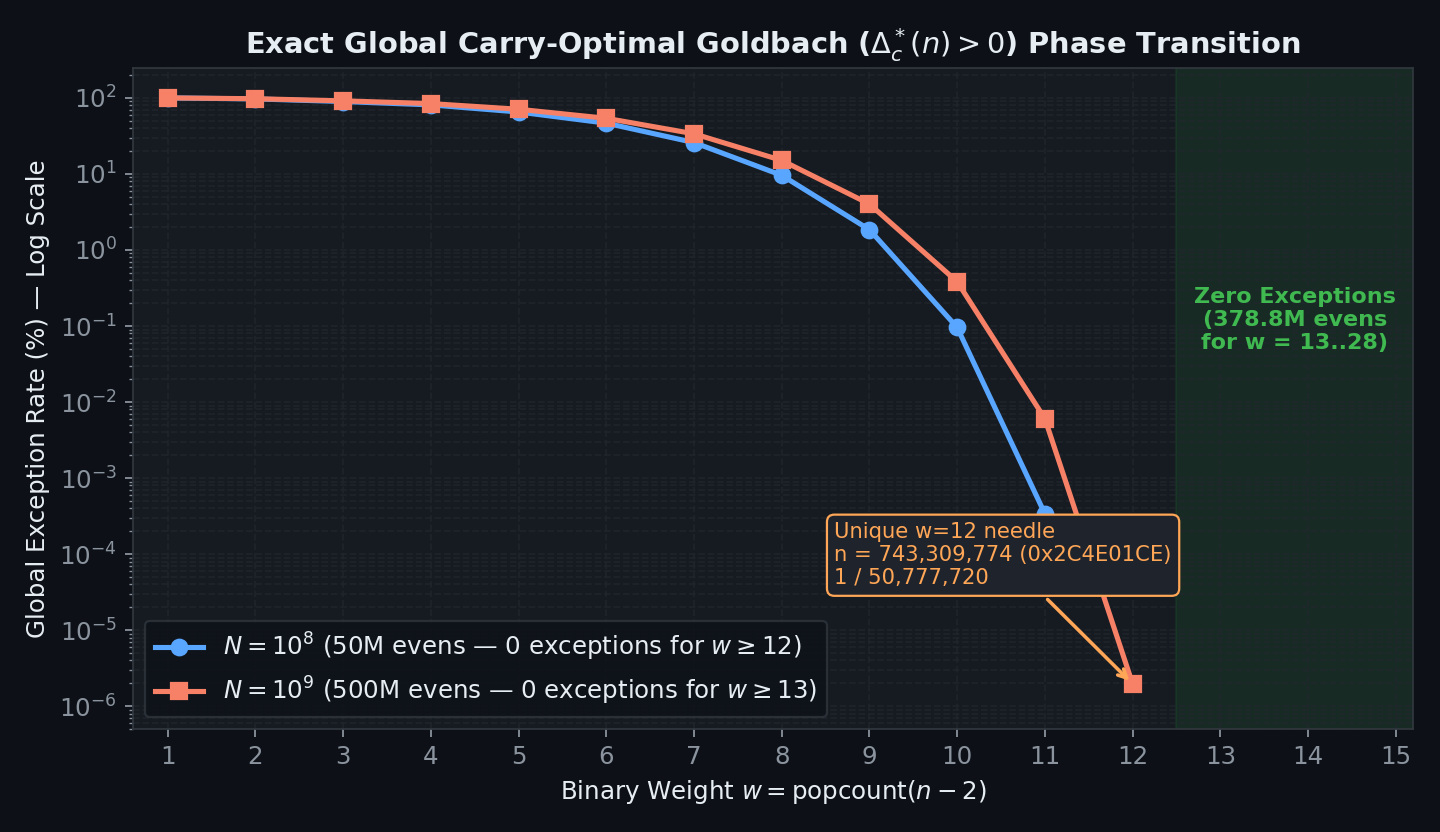
\includegraphics[width=0.85\linewidth]{../figures/carry_phase_transition.png}
\caption{Sharp binary-weight phase transition of global Carry-Optimal Goldbach exceptions at $N = 10^8$ and $N = 10^9$.}
\end{figure}

By the Prime Number Theorem, the expected number of carry-optimal prime pairs for weight $w$ scales as $\Theta(2^{w-1} / \ln^2 n)$, giving a critical threshold $w_{\text{crit}}(n) \approx 2 \log_2 \ln n$. Because a typical integer $\le N$ has $w \approx \frac{1}{2}\log_2 N \gg 2\log_2 \ln N$, we propose:

\begin{conjecture}[Sharp $\Theta(\ln \ln N)$ Threshold for Carry-Optimal Goldbach]
Combined with Theorem~\ref{thm:allw}, the extremal exception weight $W_{\max}(N)$ has exact order $\Theta(\ln \ln N)$; specifically, there exists a constant $C > 0$ such that every even integer $n$ with $\operatorname{pop}(n - 2) > \frac{2}{\ln 2} \ln \ln n + C$ satisfies $\Delta_c^*(n) = 0$, bracketing $W_{\max}(N)$ tightly inside
\[
\Bigl(\frac{1}{2} - o(1)\Bigr)\ln \ln N \;\le\; W_{\max}(N) \;\stackrel{\text{conj.}}{\le}\; \Bigl(\frac{2}{\ln 2} + o(1)\Bigr)\ln \ln N.
\]
Consequently, carry-optimal Goldbach numbers have asymptotic density $1$ among the even integers.
\end{conjecture}

\section{AVX2 Sieve Architecture and Frontier Verifications}
Our C++ engine (\texttt{goldbach.cpp}, \texttt{research\_suite.cpp}) combines: (i) a $26.2\,\text{KB}$ L1-resident byte-aligned $5$-pattern AVX2 pre-sieve eliminating all odd primes $3 \dots 47$ at $256$ bits per iteration with zero bit-shifts; (ii) an $8\times$ constant-mask unrolled wheel for primes $53 \le p < 2^{18}$; (iii) an $8$-stream L1-threshold bucket sieve for $p \ge 2^{18}$; and (iv) a $4$-prime fused AVX2 check kernel. On 12 threads, standard Goldbach is verified to $10^{12}$ in $200.8\,\text{s}$ ($4.33\text{B evens/s}$ peak at $10^{10}$, $\sim 12\,\text{MB}$ RAM, $\pi(10^{12}) = 37{,}607{,}912{,}018$ verified).

\subsection{Lemoine's Conjecture to $10^{12}$ and Twin-Prime Goldbach to $10^{10}$}
\begin{itemize}
    \item \textbf{Lemoine's Conjecture ($n = p + 2q$, odd $n \ge 7$)}~\cite{lemoine1895}: Verified deterministically for all $5 \times 10^{11}$ odd integers in $[7, 10^{12} + 1]$ in $277.8\,\text{s}$ ($1.80\text{B odds/s}$, $0$ fallbacks; $10^{10}$ in $1.146\,\text{s}$). Largest minimal $q$ up to $10^{12}$: $q = 3079$ at $n = 853{,}036{,}242{,}229 = 853{,}036{,}236{,}071 + 2 \cdot 3079$.
    \item \textbf{Twin-Prime Goldbach ($n = p + q$, both $p, q$ twin primes)}: Verified across all $5 \times 10^9$ even integers up to $10^{10}$ in $37.7\,\text{s}$ via bit-parallel twin extraction $T = B \mathbin{\&} ((B \ll 1) \mathbin{|} (B \gg 1))$. Exactly $34$ exceptions exist, the largest being $n = 4208$; the largest minimal twin witness up to $10^{10}$ is $p = 299{,}359$ at $n = 8{,}115{,}525{,}848$.
\end{itemize}

\subsection{Information Theory of Minimal Goldbach Witnesses ($N = 10^{10}$)}
Across $5 \times 10^9$ even integers up to $10^{10}$ ($38.1\,\text{s}$):
\begin{itemize}
    \item Unconditional Shannon entropy $H(p_{\min}) = 4.8616\text{ bits}$ (up $+0.181\text{ bits}$ from $10^9$).
    \item \textbf{Super-mod-6 lag-$1$ mutual information:} $I(p_{\min}(n); p_{\min}(n+2)) = 1.5872\text{ bits} > \log_2 3 = 1.5850\text{ bits}$, driven by deterministic twin-prime witness propagation $(n + 2) - (p + 2) = n - p$.
    \item \textbf{Chebyshev mod-6 witness inversion:} $p = 31$ ($4.0373\%$) occurs more frequently as $p_{\min}(n)$ than the smaller prime $p = 29$ ($3.9865\%$), due to the asymmetry of primes $\equiv 5$ vs.\ $1 \pmod 6$ below $31$~\cite{granville2006}.
\end{itemize}

\begin{figure}[h]
\centering
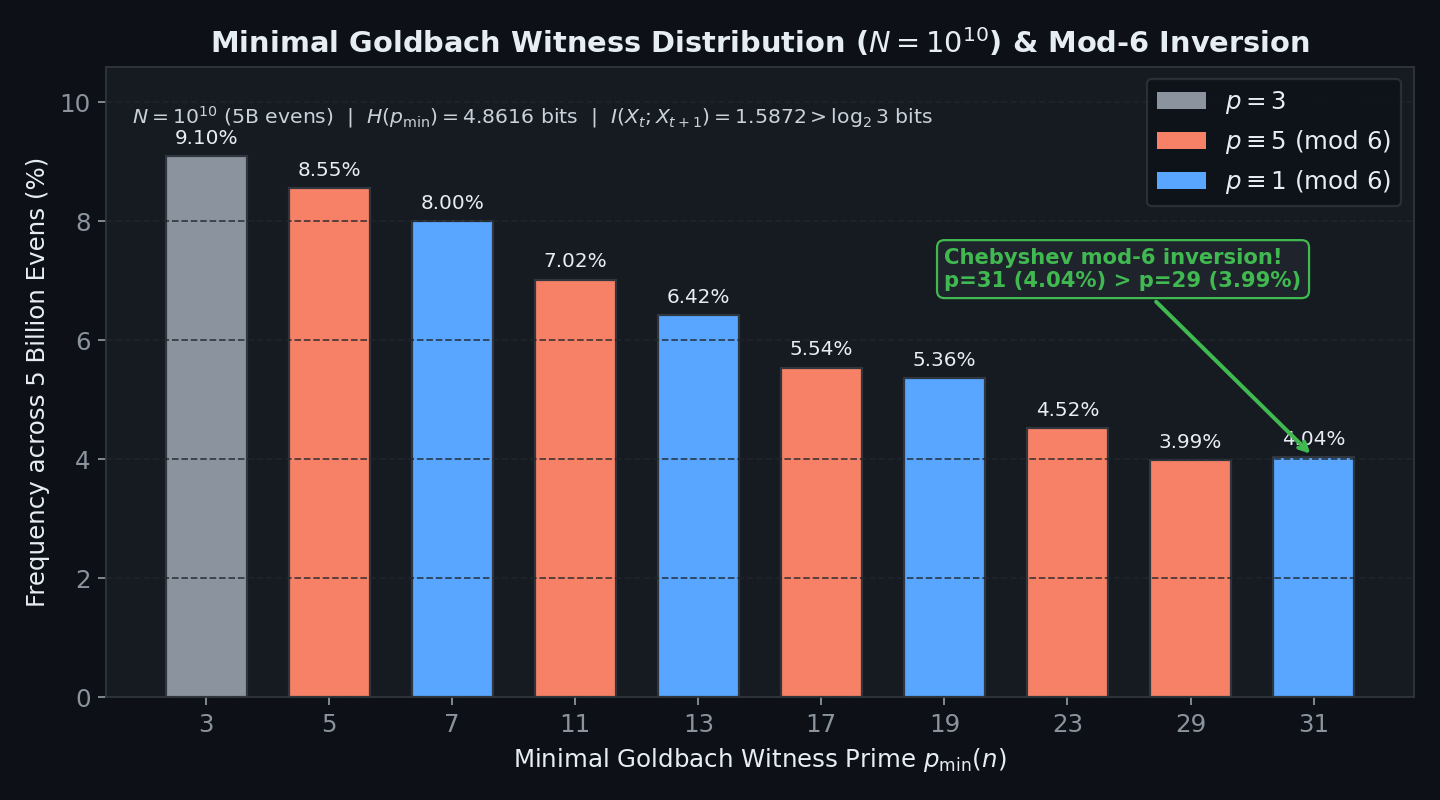
\includegraphics[width=0.85\linewidth]{../figures/witness_entropy_inversion.png}
\caption{Minimal Goldbach witness distribution across $5 \times 10^9$ even integers ($N = 10^{10}$), highlighting the Chebyshev mod-6 inversion at $p = 31 > p = 29$.}
\end{figure}

\begin{thebibliography}{9}
\bibitem{oliveira2014} T. Oliveira e Silva, S. Herzog, and S. Pardi, \emph{Empirical verification of the even Goldbach conjecture and computation of prime gaps up to $4 \cdot 10^{18}$}, Mathematics of Computation \textbf{83} (2014), 2033--2060.
\bibitem{kummer1852} E. E. Kummer, \emph{\"Uber die Erg\"anzungss\"atze zu den allgemeinen Reciprocit\"atsgesetzen}, J. Reine Angew. Math. \textbf{44} (1852), 93--146.
\bibitem{lemoine1895} \'E. Lemoine, \emph{L'interm\'ediaire des math\'ematiciens}, \textbf{1} (1894), 179; \textbf{3} (1896), 151.
\bibitem{granville2006} A. Granville and G. Martin, \emph{Prime number races}, Amer. Math. Monthly \textbf{113} (2006), 1--33.
\end{thebibliography}

\end{document}
